\subsection{选择排序}\qanswerloc{367}

\begin{qitems}
    \begin{bbox}
        \qitem 指出堆和二叉排序树的区别?
    \end{bbox}
    \begin{bbox}
        \qitem 画出一棵二叉树,使得它既满足大根堆的要求又满足二叉排序树的要求。
    \end{bbox}
    \begin{bbox}
        \qitem 若只想得到一个序列中第 $k$ ($k \ge 5$) 个最小元素之前的排序序列,
        则最好采用什么排序算法?
    \end{bbox}
    \begin{bbox}
        \qitem 通常使用的堆也称二叉堆,因为它是用完全二叉树来实现的,树中结点最多只有两个孩子。
        同理可以有 m 叉堆,即用完全 m 叉树来实现的堆。
        \begin{subqitems}
            \subqitem 下图是一个 m 叉小根堆,问 m 值是多少?向这个堆插入一个元素 65 后,
            堆中的元素如何变化?再删除堆顶元素呢?请画出变化后的树形。
            
            \begin{center}
                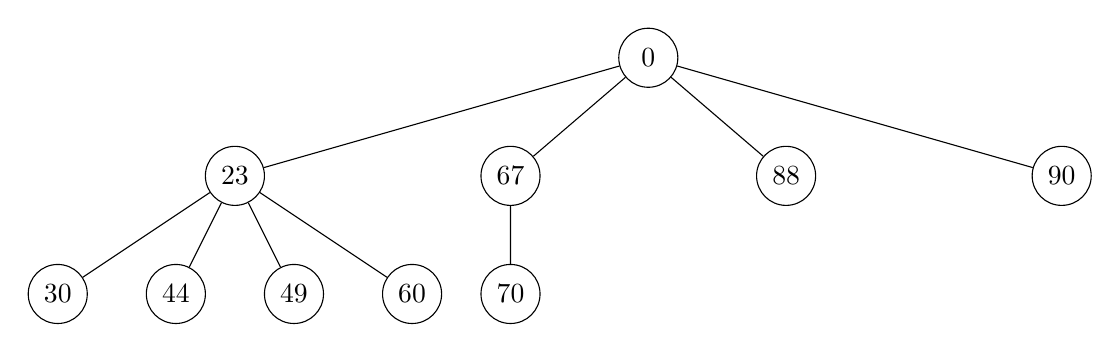
\begin{tikzpicture}[
                    level 1/.style={sibling distance=3.5cm},
                    level 2/.style={sibling distance=1.5cm},
                    every node/.style={circle, draw, minimum size=0.75cm}
                ]
                \node {0}
                    child {node {23}
                        child {node {30}}
                        child {node {44}}
                        child {node {49}}
                        child {node {60}}
                    }
                    child {node {67}
                        child {node {70}}
                    }
                    child {node {88}}
                    child {node {90}};
                \end{tikzpicture}
            \end{center}
            
            
            \subqitem 从 0 开始对完全 4 叉树中的结点从上到下、从左到右进行编号。
            若给定一个结点 $k$,其父结点的编号是多少?(若存在),其第 $i$ ($i=1, 2, 3, 4$) 个孩子的编号是多少?
            \subqitem 在 m 叉堆中进行插入和删除操作的时间复杂度是多少?
        \end{subqitems}
    \end{bbox}
    \begin{bbox}
        \qitem 编写一个算法,在基于单链表表示的待排序关键字序列上进行简单选择排序。
    \end{bbox}
    \begin{bbox}
        \qitem 试设计一个算法,判断一个数据序列是否构成一个小根堆。
    \end{bbox}
    \begin{bbox}
        \qitem 优先队列(Priority Queue)是一种数据结构,它类似于普通队列,但每个元素都有一个优先级。
        元素在入队时会根据其优先级来排序,而不按照先入先出的顺序来排序。每次从优先队列中出队时,
        出队的是优先级最高的元素,而不是最早进入队列的元素。队列中的元素的优先级的数据结构的定义如下:
        
        \quad \lstinline|typedef struct { int value; int priority; } PriorityQueueElement;| // priority 越大,优先级越高
        
        请设计一个优先队列,要求满足:\ding{172}初始时队列为空;
        \ding{173}入队时,不允许增加队列的占用空间;
        \ding{174}出队后,出队元素所占用的空间可重复使用,即整个队列所占用的空间不变;
        \ding{175}入队操作和出队操作的时间复杂度始终保持为 $O(\log n)$。请回答:
        \begin{subqitems}
            \subqitem 该队列是应选择链式存储结构,还是选择顺序存储结构?
            \subqitem 给出优先队列的数据结构的定义。
            \subqitem 用伪代码给出入队操作和出队操作的基本过程(关键之处可用文字描述)。
        \end{subqitems}
    \end{bbox}
    \begin{bbox}
        \qitem 【2022 统考真题】现有 $n$ ($n > 100000$) 个数保存在一维数组 M 中,
        需要查找 M 中最小的 10 个数。请回答下列问题。
        \begin{subqitems}
            \subqitem 设计一个完成上述查找任务的算法,要求平均情况下的比较次数尽可能少,
            简述其算法思想(不需要编程实现)。
            \subqitem 说明你所设计的算法平均情况下的时间复杂度和空间复杂度。
        \end{subqitems}
    \end{bbox}
\end{qitems} 